%!TEX root = ../LastNameI-[RnD-MT]Report.tex

\chapter{Popov-Vereshchagin Hybrid Dynamics Solver}
\label{PVS}
The previous chapter \ref{Controlscheme1}  gives an overview on modeling and controlling of robot through task based control i.e.\ by computing the required control commands which resolves the constraints imposed on the robot by task specifications. This takes into consideration the complete dynarimitmic properties of the robot. 
\par
In-order to establish task level control for tasks such as robots being in contact with environment, pushing heavy objects etc.\, the Popov Vereshchagin solver \cite{vereshchagin1974computer,popov1978manipuljacionnyje,vereshchagin1989modeling} was developed in the early 70's by E.P Popov and A.F.Vereshchagin to compute an instantaneous solution to hybrid dynamics problem (control commands) by resolving the constraints imposed on the end effector. The imposed constraints are Cartesian acceleration constraints, external force constraints from the environment, feedforward joint constraints. 
\section{Task Specification}
Based on the motivation mentioned earlier this section gives a comprehensive overview on the task specifications given to the solver. There are different types of task specifications which can be given as input to the solver. The tasks can be specified as \textit{external forces}, \textit{Cartesian accelerations} and as \textit{joint feed-forward torques}. The task specifications and their associated interfaces can be given as:
\begin{enumerate}
	\item \textbf{External force} tasks specifications defined by real or virtual forces {$F_{ext}$}.
	%given by end effector acceleration energy set point $b_{N}$
	\item \textbf{Joint} task specification which can be given by feed forward torques {$\tau$}.
	\item The \textbf{Cartesian acceleration} task specification on the end effector {$A_{N}\ddot{X}_{N} = b_{N}$}.
\end{enumerate}


The solver has the capability to take task specifications as their input and compute the control commands. The different task specifications are their uses can be noted as:
\begin{itemize}
		\item \textbf{External force $F_{ext}$} : The task specification through external forces are helpful to achieve tasks with situations where the manipulator in contact with the environment or while performing reconfiguration of robot. They are also useful in tasks involving impedance control.
		\item \textbf{Feed-forward joint torques $\tau$}: The task specification through joint torques is useful for handling situations with joint limit avoidance where these constraints act as virtual spring by pushing away from singularities when the limits are close to singularity, null space motion.
\item \textbf{The Cartesian acceleration $A_{N}\ddot{X}_{N} = b_{N}$}: The task specification through Cartesian acceleration constraints can also be useful to tasks involving manipulators being in contact with the environments or to perform tasks such as manipulation by specifying accelerations on end effector. These can be specified in the form of physical or virtual constraints. The solver requires the user to specify the directional information of the constrained acceleration and the amount of acceleration energy applied in that particular direction.


Thus the constraints specified on the end effector segment can be given as: ~\cite{shakhimardanov2015composable} 
	\begin{equation}
	A_{N}^{T}\ddot{X}_{N} = b_{N}
	\end{equation} 
	
	
The columns of $A_{N}$ represent that the directions in which the segment is constrained. The vector $b_{N}$ signifies the acceleration energy set points (amount of acceleration) in each direction. Depending on the number of constraints (m), the dimensions of matrix $A_{N}$ and vector $b_{N}$ will be $6\times m$ and $m\times 1$ respectively.
	
	
The constraints specified by the user, can be complete or partially stated in such a way that the they are less than $m$ number of constraints. For eg: constraining the motion of the end effector/segment in linear z and angular x directions. This means that the robot cannot accelerate in linear z and angular x directions, rest of the directions remain unconstrained. The unit constraint matrix for this case can be defined as \cite{shakhimardanov2015composable}:
	\[A_{N} =
	\begin{bmatrix}
	0 & 0 \\ 0 & 0 \\ 1 & 0 \\ 0 & 1 \\ 0 & 0 \\ 0 & 0
	\end{bmatrix} \;\;\;
	b_{N} =
	\begin{bmatrix}
	0 \\ 0
	\end{bmatrix}
	\]
	
	
In the above case the initial three rows of the unit constrained force matrix ($A_{N}$) allow to specify the linear constraints in \textit{x}, \textit{y} and \textit{z} directions and similarly the lower three rows specify angular constraints in the respective directions. The acceleration energy ($b_{N}$) has been set to zero which indicates the robot does not produce any acceleration energy in these particular directions. 
	
	
Considering an additional case indicating complete specification of acceleration constraints. By constraining all the \textit{six} directions of the end effector, an identity matrix of size $6 \times 6$ is obtained as in: ~\cite{shakhimardanov2015composable}
	\[	A_{N} =
	\begin{bmatrix}
	1 & 0 & 0 & 0 & 0 & 0\\ 0 & 1 & 0 & 0 & 0 &0\\ 0 & 0 & 1 & 0 & 0 & 0\\ 0 & 0 & 0 & 1 & 0 & 0\\0 & 0 & 0 & 0 & 1 & 0\\ 0 & 0 & 0 & 0& 0 &1
	\end{bmatrix}  \;\;\;
	b_{N} =
	\begin{bmatrix}
	\ddot{X}_{N}
	\end{bmatrix}
	\]
	
	
Since $A_{N}$ is an identity matrix, the magnitudes of two vectors representing Cartesian accelerations ($\ddot{X}_{N}$) and acceleration energy set point ($b_{N}$) both of dimensions $6\times 1$ are being assigned to each other, in spite of their difference in their physical units. This means that in this scenario, the $A_{N}\ddot{X}_{N} = b_{N}$ where $A_{N}$ represents unit forces, the magnitudes of acceleration energy and acceleration match up. This signifies that the acceleration energy is produced by constraint forces which is dealt for each of the directional constraints. In the above scenario, every column of unit constrained force matrix indicate a value of $1$ which indicates the direction of the constrained force. Similarly the value of Cartesian acceleration is equal to the acceleration energy set point in the respective directions of the constrained forces ~\cite{vukcevic2018extending}.


By the definition of hybrid dynamics we calculate the unknown forces and accelerations with given forces and accelerations at joints. The solution to the Popov Vereshchagin solver is given by $\ddot{q}$ (joint accelerations), $\tau_{ctrl}$ in joints and $\ddot{X}$ (Cartesian accelerations) on links. Since hybrid dynamics solver is a combination of both forward and inverse dynamics solvers. The results $\ddot{q}$ and $\ddot{X}$ are provided as solution to forward dynamics solver and the $\tau_{ctrl}$ for inverse dynamics solver. 
\end{itemize}

\begin{figure}[h!]
	\centering
	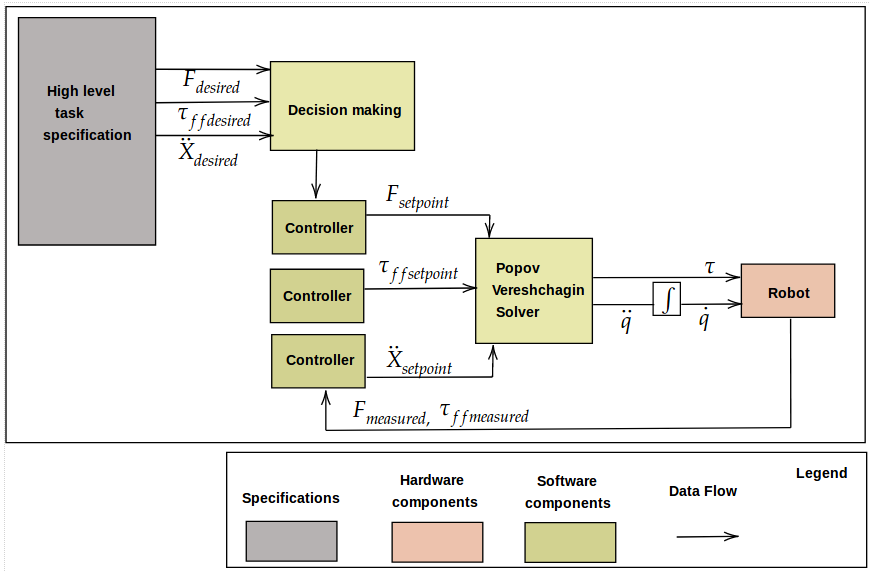
\includegraphics[width=0.9\textwidth]{images/algo1}
	\caption{Schematic representation of task level specification in Popov Vereshchagin solver}
	\label{Controlscheme1}
\end{figure}

\section{Functionality of the solver}
In general the term \textit{solver} can be defined as the one which is able to solve a differential equation (equations of Constrained motion), where optimal control problem(OCP) is one of the special cases of differential equations \color{red}\cite{write this}\color{black}. There are special cases of differential equations and OCP's which can be resolved analytically instead of using numerical techniques. Hence, Popov Vereshchagin solver can be categorized one among them. The solvers can be categorized into domain specific solvers and domain independent solvers. The domain specific solvers use optimization techniques and specific to a particular domain. Examples of such solvers are ABA, ACHD, Newton-Euler ~\cite{shakhimardanov2015composable}. The domain independent solvers solve OCP using numerical methods ~\cite{shakhimardanov2015composable}. The Popov Vereshchagin solver is also a domain specific solver. The solver performs recursion over kinematic tree, the search space is reduced by the structure of the kinematic tree.


The main functionality of the solver is that it computes the system's constrained motion. As mentioned in \cite{vereshchagin1989modeling} this solver is based on \textit{Gauss's principle of least constraint} which belongs to the variational principles of classical mechanics. It states that the real motion (constrained motion) of the system is determined by minimum of the convex function which are subjected to linear constraints ~\cite{vereshchagin1989modeling}\cite{gauss1829neues}\cite{vukcevic2018extending}. It indicates that in a constrained system inorder to find the true accelerations of masses, the accelerations are initially computed by treating them as unconstrained and then projecting them onto the nearest accelerations which satisfy the constraints \cite{gauss}. 


The Gauss function which is minimized is thus given as ~\cite{vereshchagin1989modeling}:
\begin{equation}
\label{Gauss}
\min_{\ddot{q}} Z (\ddot{q}) = \sum_{i=0}^{N}\frac{1}{2}\ddot{X}_{i}^{T}H_{i}\ddot{X}_{i} + F_{bias,i}^{T}\ddot{X}_{i}+ \sum_{j=1}^{N}\frac{1}{2}d_{j}\ddot{q}_{j}^{2} - \tau_{j}\ddot{q}_{j}
\end{equation}


where $Z$ is defined as the Zwang (Degree of constraint), $H_{i}$ is the rigid body inertia which is a symmetric matrix of size $6\times 6 $, $\ddot{X}$ represents a $6\times 1$ vector for Cartesian accelerations of particular robot links. $F_{bias,i}$ represents the effects of external forces, Coriolis and centrifugal forces, which is collectively called as bias force which is a vector of size $6\times 1$ , $\tau_{j}$ the feed-forward joint torques, $d$ represents the inertia of the \color{red}motor actuating the joint \color{black}rotor \cite{vereshchagin1989modeling}. 


The Gauss function is subjected to \cite{vukcevic2018extending}: 
$$
\ddot{X}_{i+1} = {^{i+1}X_{i}} \ddot{X}_{i} + S_{i}\ddot{q}_{i+1}+ \ddot{X}_{bias,i+1}$$
$$A_{N}^{T}\ddot{X}_{N} = b_{N}$$


In the above equation $A_{N}$ represents matrix of unit constraint forces. As mentioned earlier they contain the direction of the acceleration constraints. $b_{N}$ denotes the vector of acceleration energy set point for segment N.


Reformulating the equation \ref{Gauss} in-order to account for acceleration constraints on segments as: 
\begin{equation}
\min_{\ddot q,\nu}   Z(\ddot{q},\nu)  = \sum_{i=0}^{N}\frac{1}{2}\ddot{X}_{i}^{T}H_{i}\ddot{X}_{i} +  \sum_{j=1}^{N}\frac{1}{2}d_{j}\ddot{q}_{j}^{2} - \tau_{j}\ddot{q}_{j} + \nu^{T}A_{N}^{T}\ddot{X}_{i}
\label{Gaussaian}
\end{equation}


The above equation uses the method based on Lagrange equations ~\cite{shakhimardanov2015composable}\cite{lagrange1853mecanique}. $\nu$ represents the Lagrange multiplier (magnitude of constraint forces). Using Bellman's principle of optimality the iterative formulation of equation \ref{Gaussaian} has been converted to recursive formulation \cite{bellman1952theory}.


The solution to the Popov Vereshchagin solver is \textit{joint accelerations} ($\ddot{q}$). The solver also finds magnitude of \textit{constraint forces} ($\nu$) and \textit{Cartesian accelerations} ($\ddot{X}_{i}$).


The Popov Vereshchagin solver has been derived from \textit{Gauss Principle}. The underlying working principle for the Popov Vereshchagin solver can be represented as:
\begin{equation}
F_{c} = A_{N}\nu
\end{equation}
$$ \nu = \frac{F_{c}}{A_{N}} =  \frac{E_{present}}{E_{required}}$$ 
where $F_{c}$ is a force constraint and $A_{N}$ is the directional constraint and the $\nu$ is Lagrange multiplier which is equivalent to applying $E_{present}$ which is the current acceleration energy which is generated by bias forces, external forces or joint torques and and $E_{required}$ is the acceleration energy which is required to satisfy the constraints in Popov Vereshchagin solver. Since both the energies can be calculated and $\nu$ can be derived as a result of this. Constantly scaling constraint directions will allow computation of $F_{c}$.\\
\indent
The input requirements to the solver are the kinematic chain model parameters, joint angles and joint velocities at the current time instant, feedforward joint torques, the external forces applied to individual segments and $A_{N}$ is the desired constraint (unit force) applied and $b_{N}$ is the desired acceleration energy set point on the end effector respectively. \\
\indent
The Popov Vereshchagin algorithm is a three pass/sweep algorithm. The algorithm performs two outward and one inward computational sweep on the kinematic chain \cite{shakhimardanov2015composable}. The first is the outward sweep that controls the calculation of pose, velocity and bias terms from the root of the robot (base) to the leaves (end effector). Then, the inward sweep is involved in calculation of articulated-body inertias and joint forces. The last sweep is another outward sweep again, which calculates the end result of joint torques, joint accelerations and Cartesian accelerations for each segment \cite{shakhimardanov2015composable}. In addition to the above calculations, the solver after the second recursion computes the magnitude of constraint forces (Lagrange multiplier), which is performed when the solver visits the base segment. This hybrid dynamics solver has the run time complexity of $O(n)$ where n is the number of segments, as the solver visits every segment only one time. 
\\
\begin{algorithm}[H] \label{alg1}
%	\TitleOfAlgo{Constrained Hybrid Dynamics Solver}
	\SetAlgoLined
	\SetKwInOut{Input}{Input}
	\SetKwInOut{Output}{Output}
	\Input{\ $\mathbf{Kin \ Chain \ model, \ q, \ \dot{q}, \ \mathbf{\mathlarger{\mathlarger{\tau}}}, \ \ddot{X}_0, \ F_{ext}, \ A_N, \ b_N}$}
	\Output{\ $\mathbf{\mathlarger{\mathlarger{\tau_{\textbf{ctrl}}}}}, \ \mathbf{ \ddot{q}, \ \ddot{X}}$}
	
	\SetKwBlock{Begin}{begin}{end}
	\Begin{
	{
		\For{$\mathbf{i \ = \ 0 \ \ to \ \ N-1}$}{
			${}^{i+1}_{i}X = ({}^{d_i}_{i}X \ \  {}^{i+1}_{d_i}X(q_i))$\; \label{alg:pose}
			\vspace{1mm}
			${\dot{X}_{i+1} = {^{i+1}X_{i}} \dot{X}_i + S_{i+1} \dot{q}_{i+1}}$\; \label{alg:velocity}
			\vspace{1mm}
			${\ddot{X}_{bias,i+1} = {\dot{X}_{i+1}} \times S_{i+1} \dot{q}_{i+1}}$\; \label{alg:bias_acc}
			\vspace{1mm}
			${{F}^{A}_{bias,i+1} = {\dot{X}_{i+1}} \times^* H_{i+1} \dot{X}_{i+1} - {^{i+1}X_{0}^*}  {F}^{ext}_{0,i+1}}$\; \label{alg:bias_force1}
			\vspace{1mm}
%			${F_{bias,i+1} = {F_{bias,i+1} - {^{i+1}X_{0}^*} \ {F}^{ext}_{0,i+1}}}$\; \label{alg:bias_force}
		%	\vspace{1mm}
			${H_{i+1}^A = H_{i+1}}$\; \label{alg:I_A}
		%	${{F}^{A}_{bias,i+1} = F_{bias,i+1}}$\; \label{alg:bias_force_A}
	}	
		 $L_{N} = 0, U_{N} = 0$\\
		
		\vspace{2mm}
%		{
		\For{$\mathbf{i \ =  \ N-1  \ \ to \  \ 0}$}{
			${D_{i+1} = d_{i+1} + S_{i+1}^T H_{i+1}^A S_{i+1} }$\; \label{alg:sum_inertia}
			\vspace{2mm}
			${P_{i+1} = 1 - H_{i+1}^AS_{i+1} D_{i+1}^{-1} S_{i+1}^{T}}$\; \label{alg:P}
			\vspace{2mm}
			${H_{i+1}^a = P_{i+1} H_{i+1}^A}$\;
			\label{alg:I_a}
			\vspace{2mm}
			${H_i^A = H_i^A + {^{i}X_{i+1}^*} H_{i+1}^a {^{i}X_{i+1}}}$\; \label{alg:I_A2}
			\vspace{1mm}
			${F_{bias,i+1}^a = P_{i+1}^A F_{bias,i+1}^A + H_{i+1}^AS_{i+1} D_{i+1}^{-1} \tau_{i+1}+ H_{i+1}^a\ddot{X}_{bias,i+1}}$\; \label{F_bias_a}
			\vspace{2mm}
			${F_{bias,i}^A = F_{bias,i}^A + {^{i}X_{i+1}^*} F_{bias,i+1}^a}$\; \label{F_bias_A}
			\vspace{2mm}
			${A_i = {^{i}X_{i+1}^*} P_{i+1}^A A_{i+1}}$\;  \label{alg:A_i}
			\vspace{2mm}
			${U_i = U_{i+1} + A_{i+1}^T \{\ddot{X}_{bias,i+1} + S_i D^{-1}_i(\tau_{i+1} - S_i^T(F_{bias,i+1}^A + H_{i+1}^A \ddot{X}_{bias,i+1}))\}}$\; \label{alg:U_i}
			\vspace{-4mm}
			${\mathcal{L}_i = \mathcal{L}_{i+1} - A_{i+1}^T S_{i+1}D^{-1}_{i+1} S_{i+1}^T A_{i+1}}$\; \label{alg:L_i}
		}
		
%		\vspace{2mm}
%		%// Balance of acceleration energy at the base (\{0\} link)\\
%%		// Computation of Lagrange multiplier\\[2mm]
		$\nu = {\mathcal{L}_0^{-1}(b_N - A_0^T \ddot{X}_0 - U_0)}$\; \label{alg:balance}
		\vspace{3mm}
%		
%%		{// Outward sweep for torques and acceleration}\\
		\For{$\mathbf{i \ = \ 0  \ \ to \ \ N-1}$}{
			${\ddot{q}_{i+1} = D^{-1}_{i+1}\{\tau_{i+1} - S^T_{i+1} (F_{bias,i+1}^A + H_{i+1}^A ({^{i+1}X_{i}} \ddot{X}_i + \ddot{X}_{bias,i+1}) + A_{i+1}\nu)\}}$\; \label{alg:q_acc}
			\vspace{-4mm}
			${\ddot{X}_{i+1} = {^{i+1}X_{i}} \ddot{X}_i  + \ddot{q}_{i+1} S_{i+1} + \ddot{X}_{bias,i+1}}$\; \label{alg:X_acc}
	}
	}
}

	\caption{Popov Vereschchagin Hybrid Dynamics Solver \cite{vereshchagin1989modeling, popov1978manipuljacionnyje, shakhimardanov2015composable, vukcevic2018extending}}
	
\end{algorithm}

\section{Comprehensive explanation of the solver}
\label{comprehensivesolver}
\begin{figure}[h!]
	\centering
	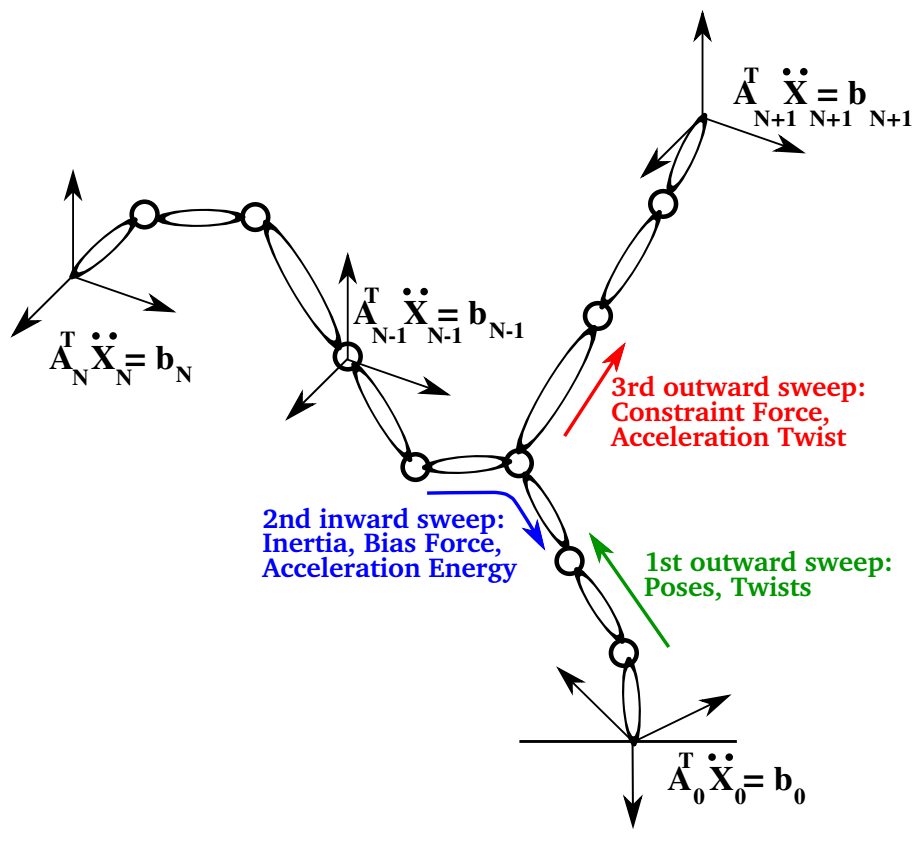
\includegraphics[scale=0.3]{images/solver1}
	\caption{Sweeps present in Popov Vereschchagin solver \cite{shakhimardanov2015composable}} 
\end{figure}
\begin{itemize}
	\item \textbf{Outward sweep} : The first outward sweep performs recursion of position, velocity and bias acceleration.
	
	
The line \ref{alg:pose} of the algorithm performs the calculation of pose relation between the links \{i+1\} and \{i\} i.e.\ calculation of pose on proximal frames of segment \{i+1\} w.r.t segment \{i\}. This can be seen in figure \ref{Segment Transformation}.
%	This is formed as the given equation as in \cite{shakhimardanov2015composable}:
	\begin{figure}
		\centering
		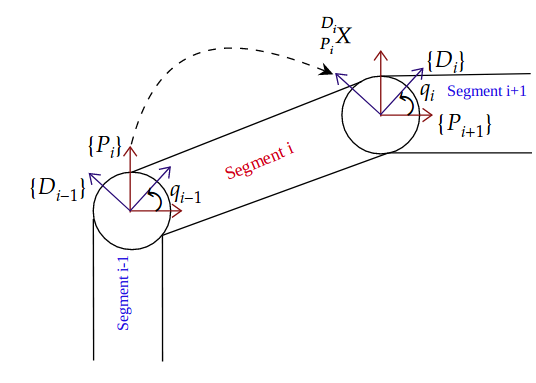
\includegraphics[scale=0.6]{images/segment_pose2}
		\caption{Frames and transformations assignment between segments in kinematic chain}
		\label{Segment Transformation}
	\end{figure}
The pose calculation as mentioned above is given by composing transformations of ${}^{D_{i}}_{P_{i}}X$, between proximal and distal frames of segment {i} and transformations of ${}^{P_{i+1}}_{D_i}X(q_i)$ between proximal frame of link {i+1} and distal frames of link {i} and also shows its dependence of joint position variable $q_{i}$ \cite{shakhimardanov2015composable}. 


In order to find the Cartesian velocity as in line \ref{alg:velocity} i.e.\ $\dot{X}$ of segment i+1, it requires contribution from the joint velocity twist $\dot{X_{i}}$ along with joint velocity $\dot{q}_{i+1}$. The expression uses $S$ which is the motion subspace matrix which represents constraining every joints motion to motion subspace ~\cite{featherstone2014rigid}. Also the term ${}^{i+1}X_{i}$ indicates a co-ordinate transformation of motion vector (refer \ref{Spatial}) relating co-ordinates between \{i\} and \{i+1\} ~\cite{shakhimardanov2015composable}.


Given the velocity twist and joint rate of link \{i+1\}, the line \ref{alg:bias_acc} denotes the calculation the linear and angular components of bias acceleration $\ddot{X}_{bias,i+1}$. The detailed expression uses the property of spatial cross product operator (refer \ref{cross}).
%The above expression will only be calculated when joint acceleration is known, which is true only in case of inverse dynamics where forces/moments of force are computed with given desired segment motions. But in the case of forward dynamics , it is necessary to compute the desired segment motions, when the given are the desired forces\cite{shakhimardanov2015composable}. \\


Later, in the consecutive step the solver computes bias force vector $F_{bias,i+1}$, which is calculated given spatial velocity twist $\dot{X}_{i+1}$and rigid body inertia $H_{i+1}$. The external forces are taken into account and the effect of applying these external forces are subtracted from the bias force vector of segment \{i+1\}. The expression ${}^{i+1}_{0}X^*$ is matrix representation of change of coordinates of force vector between ${0}$ to ${i+1}$ refer \ref{Spatial} \cite{vukcevic2018extending} which means $F^{ext}_{0,i+1}$ are measured in frame \{i+1\} but is expressed in base frame {0} ~\cite{shakhimardanov2015composable}.

%		
%\subsection{Inward Sweep}
The lines \ref{alg:I_A} and \ref{alg:bias_force1} indicate initial initializations of respective rigid body values to \textit{articulated rigid body inertia} matrix and \textit{bias force} vector.

\item \textbf{Inward Sweep}: During the inward sweep the algorithm deals with calculation of articulated body quantities. 
%The calculations are performed in a loop for each value of \{i\} from $N-1$ down 0 \cite{featherstone2014rigid}. 


The line \ref{alg:sum_inertia} is given as the joint space inertia of segment \{i+1\} added along with the joint rotor of segment \{i+1\}. The line \ref{alg:P} defines the \textit{projection matrix} of segment \{i+1\}, for inertias and forces of the articulated body over the joint axis. The projections are over the joint axis. The next steps (see lines \ref{alg:I_a}, \ref{alg:I_A2}) define \textit{articulated body inertia} and \textit{apparent body inertia} which are summed up from all children segments in the kinematic chain. Similarly, summing up bias forces transmitted by children segments as $F_{bias}^{a}$ (see line \ref{F_bias_A}) contribute to the \textit{articulated body bias forces} \cite{vukcevic2018extending}.


Due to the specification of end effector constraints the unit forces are felt or experienced on every segment.
The line \ref{alg:A_i} in the algorithm calculates the unit constraint forces which have been propagated and experienced on the segment \{i\} because of the specification of the end effector constraints. The term $A$ represents a unit constraint force matrix of dimension $6\times m$ where m is the number of constraints and indicates the direction of the acceleration constraint. However, the magnitude of constraint forces are still unknown in this step.
%These can be in linear and angular directions and calculated in equation \ref{alg:A_i}.\\


The next subsequent line \ref{alg:U_i} defines the matrix $U_{i}$ which accumulates the generated (present) acceleration energy which has been generated by external forces, joint torques and contributions from inertial forces over recursive computation from end effector segment to the segment \{i\}. 
%indicates the recursive computation of amount of acceleration energy which has been generated by existing feedforward torques and also contribution from bias forces.
%of forces that the solver is expected to calculate. That indicates the matrix takes into account the amount of acceleration energy which has been produced by existing feedforward torques and also contribution from bias forces.
%As mentioned in \cite{shakhimardanov2015composable}, the inward sweep monitors "...how much of desired constraint acceleration energy i.e.\ $b_{N}$" has already been generated by the $F_{ext}$ and also by the torques applied on joints \cite{shakhimardanov2015composable}. 


The aforeknown contribution of generated acceleration energy need not additionally contribute to the constraint forces which is to be calculated in the balance equation. The matrix $U_{N}$ is initialized to 0. The line \ref{alg:L_i} represents $\mathcal{L}_{i}$ called the constraint coupling matrix initialized to 0. This keeps monitoring the desired acceleration energy which is required by the unit constraint forces. If the specified constraints on the end effector are not achievable by the kinematic chain i.e if the robot has lesser DOF's than it is required for the task. In such cases the constraint coupling matrix loses its rank. The run time singularity cannot be detected in the current state of the art of the Popov Vereshchagin solver. The basic solution presented by \cite{shakhimardanov2015composable} on the solver as a solution to singularity is weighted least square method. The early detection of singularity has been worked upon and evaluated as in \ref{Approach}. 


The core of the algorithm represented by line \ref{alg:balance} lies in the computation of the magnitude of constraint forces (Lagrange multiplier $\nu$) balances the between the desired acceleration energy which has already been generated and acceleration energy which is required for the task.
%Thus the equation allows computation of magnitude of constraint forces $\nu$.	

%The last outward sweep calculates the solution to the problem \ref{Controlscheme1} which computes torques and cartesian accelerations as the end result.\\
\item \textbf{Outward Sweep}: The final outward sweep provides the solution to equation \ref{Gaussaian} where joint accelerations and control torques are calculated. The resulting control torque is a combined effect of feed-forward torques, torques due to bias forces, and also torques generated due to constraint forces. This represents line \ref{alg:q_acc} the real/true acceleration of constrained motion. This can be given as in \cite{vereshchagin1989modeling}:
	\begin{equation}
			{\ddot{q}_{i+1} = D^{-1}_{i+1}\{\overbrace{\underbrace{\tau_{i+1}}_{\tau_{ff}} - \underbrace{S^T_{i+1}A_{i+1}\nu}_{\tau_{constraint}} -\underbrace{S^T_{i+1} (F_{bias,i+1}^A + H_{i+1}^A ({^{i+1}X_{i}} \ddot{X}_i + \ddot{X}_{bias,i+1})\}}_{\tau_{bias}}}^{\tau_{ctrl}}}\label{outwardsweep2}
	\end{equation}
	%Hence in forward dynamics the joint torques are known and thus the joint accelerations can be easily derived from the above equation.
From the above results, finally the Cartesian acceleration is calculated for every segment represented in line \ref{alg:X_acc}.

%The observation that can be made is that the true accelerations which minimize the acceleration energy result in a real motion and this is calculated by the solver \cite{bruyninckx2000gauss}. According to Gauss's principle the real constrained motion(acceleration) of a system will be ``..``closest possible acceleration to its unconstrained motion(acceleration)``~\cite{redon2002gauss}. As seen in equation \ref{outwardsweep2} the constrained motion is contributed by the three forces, namely $\tau_{constraint}, \tau_{ff}$ and $\tau_{bias}$ where the $\tau_{bias}$ can be given by external contributions of gravity and centrifugal and Coriolis forces and the $\tau_{ff}$ stands for feedforward torques. The unconstrained/free motion is represented by $\tau_{ff}$ and $\tau_{bias}$ in the equation \ref{outwardsweep2} ~\cite{vukcevic2018extending} these are the existing and applied forces in the system. 

%\section{Constraint Specification}
%This section explains the specification of constraints or how the task can be specified in Popov-Vereshchagin solver. There constraints which can imposed on a Hybrid Dynamics algorithm are:
%\begin{enumerate}
%	\item $F_{ext}$ resulted from real or virtual force constraints.
%	\item Joint constraints can be given by feed forward torques $\tau$ through which tasks can be specified.
%	\item The acceleration constraints given by end effector acceleration energy set point $b_{N}$ \cite{Marieke-Report}
%\end{enumerate}
%The constraints which are specified on the end effector segment should fulfill this equation as in \cite{shakhimardanov2015composable} 
%$$A_{N}^{T}\ddot{X}_{N} = b_{N}$$ 
%The above equation is "linearly constrained"\cite{shakhimardanov2015composable}. Depending on the number of constraints(m) the dimension of matrix $A_{N}$ will be $6\times m$ which is called unit constrained force matrix and the matrix $b_{N}$ will be $m\times 1$ vector which is called acceleration energy. The columns of $A_{N}$ represent that the directions in which the segment is constrained. The constraints can be specified by the user, where it can be completely stated by the end user or partially stated in such a way that the they are less than m. For eg: constraining the motion of the end effector/segment in linear z and angular x directions, then we can define the unit constraint matrix to be \cite{shakhimardanov2015composable}
%\[
%\begin{bmatrix}
%	A_{N} 
%\end{bmatrix}
%=
%\begin{bmatrix}
%	0 & 0 \\ 0 & 0 \\ 1 & 0 \\ 0 & 1 \\ 0 & 0 \\ 0 & 0
%\end{bmatrix},
%\begin{bmatrix}
%b_{N}
%\end{bmatrix}
%=
%\begin{bmatrix}
% 0 \\ 0
%\end{bmatrix}
%\]
%The first three rows of the constraint specification matrix allow to specify the linear constraints in x,y and z directions and similarly the lower three rows specify for angular constraints in the respective directions. These constraints indeed restrict the robot from achieving its motion in these directions, also acceleration energy has been set to zero which indicates the robot does not produce any acceleration energy in these particular directions. 
%\par Lets consider another case where we specify both linear and angular constraints. We apply this to 5 DOF manipulator, hence we mention only five constraints. The end effector/segment is allowed motion in all directions except in  angular z as in \cite{shakhimardanov2015composable}
%\[
%\begin{bmatrix}
%A_{N} 
%\end{bmatrix}
%=
%\begin{bmatrix}
%1 & 0 & 0 & 0 & 0\\ 0 & 1 & 0 & 0 & 0\\ 0 & 0 & 1 & 0 & 0\\ 0 & 0 & 0 & 1 & 0\\0 & 0 & 0 & 0 & 0\\ 0 & 0 & 0 & 0& 0
%\end{bmatrix},
%\begin{bmatrix}
%b_{N}
%\end{bmatrix}
%=
%\begin{bmatrix}
%0 \\ 0 \\ 0 \\0 \\0
%\end{bmatrix}
%\]
%Finally, constraining all 6 directions of the end effector, we get an Identity matrix of size $6 \times 6$ as in \cite{shakhimardanov2015composable}
%\[
%\begin{bmatrix}
%A_{N} 
%\end{bmatrix}
%=
%\begin{bmatrix}
%I_{6\times 6}
%\end{bmatrix},
%\begin{bmatrix}
%b_{N}
%\end{bmatrix}
%=
%\begin{bmatrix}
%\ddot{X}_{N}
%\end{bmatrix}
%\]
%Here, we assign the spatial acceleration vector to acceleration energy vector, even though they differ in their physical units. This signifies that the acceleration energy is produced by constraint forces which is dealt for each of the directional constraints. Hence, a single value specification in each individual columns of matrix $A_{N}$ suggest that the constraint force works only in that particular direction. "In turn follows that value of acceleration energy is the same as value of acceleration, in respective direction" \cite{vukcevic2018extending}
%\par 
%%The tasks can also be specified as feedforward torques which is given as the input to the solver.
%By the definition of hybrid dynamics we calculate the unknown forces and accelerations with given forces and accelerations at joints. The solution to the Vereshchagin solver is given by $\ddot{q}$ (joint accelerations), $\tau_{ctrl}$ in joints and $\ddot{X}$ (cartesian accelerations) on links. Since hybrid dynamics solver is a combination of both forward and inverse dynamics solvers. The results $\ddot{q}$ and $\ddot{X}$ are provided as solution to forward dynamics solver and the $\tau_{ctrl}$ for inverse dynamics solver. 
%	\begin{figure}
%		\centering
%		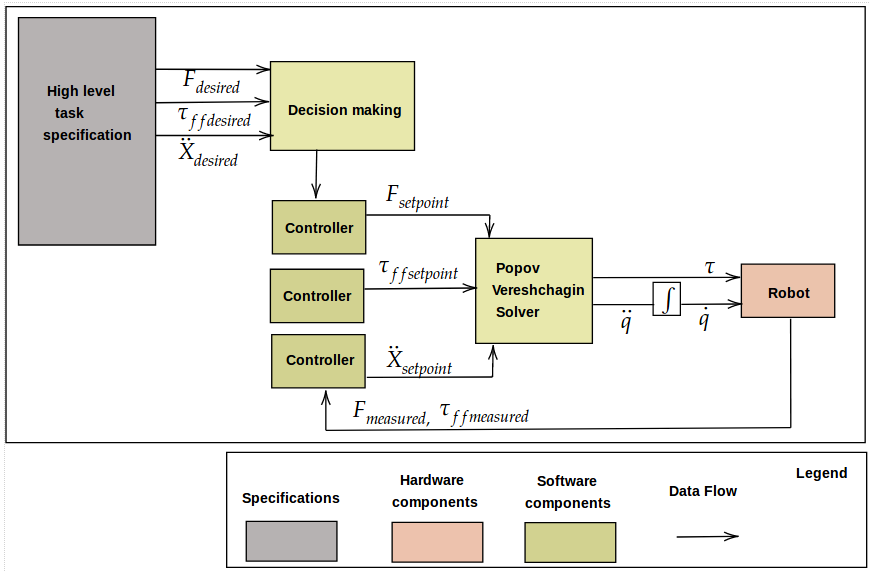
\includegraphics[width=0.8\textwidth]{images/algo1}
%		\caption{Schematic representation of task level specification in Popov Vereshchagin solver}
%			\label{Controlscheme1}
%	\end{figure}
\end{itemize}
\section{Summary}
The current implementation Popov Vereshchagin algorithm is provided in OROCOS Kinematics and Dynamics library (KDL) \cite{kdl}. This is an open source library and the computer language is C++ in which the complete library has been implemented.


This algorithm was implemented mainly by Ruben Smits, Herman Bruyninckx, and Azamat Shakhimardanov. For the tasks to be executed safely and to be monitored during the runtime the user should implement software mechanism externally. Inorder to or provide an extension to the solver in the case of singularity, where the constraint coupling matrix $\mathcal{L}$ becomes rank deficient which can be due to many reasons. The KDL library does not provide the user useful information for debugging. 


The work by Shakhimardanov on Popov-Vereschagin also provides extension to be able to apply multiple constraints on different or same segments/end effector in tree structured kinematic chains \cite{shakhimardanov2015composable}. Due to the above mentioned reasons, this algorithm has been of great interest and benefit to the robotics community. 

%\subsection{control torques and external forces}
%\subsection{Implementation and Summary}